\documentclass[11pt,sort]{jarticle}
\usepackage{latexsym}
\usepackage{mathrsfs}
%\usepackage{url}
%\usepackage{lscape}
\usepackage{graphics}
\usepackage{theorem}

\newtheorem{caution}{注意}

%% for apple LaserWriter Series %%
%% 
\setlength{\topmargin}{-0.5in}
\setlength{\textwidth}{5.6in}
\setlength{\textheight}{8.8in}
\setlength{\oddsidemargin}{0.35in}
\setlength{\evensidemargin}{0in}

\usepackage{theorem}
\renewcommand{\baselinestretch}{1.2}
\setlength{\parskip}{0.25ex}
\renewcommand{\arraystretch}{0.85}

\title{光電効果とプランク常数の決定}
\author{下薗 真一}
\date{暫定板 27 Apr. 2015}

\begin{document}

\maketitle

\section{光電効果}

多くの金属で,表面に光(電磁波)をあてると電子が飛び出す現象がおきる.
これは光電効果 photoelectric effect とよばれる.

電磁波はマクスウェルによってその存在を方程式から予測されていた.
ヘルツ H. Hertz はこれを確かめる試みの中で,この光電効果を 1887 年に発見した.
しかしその現象は,光を波動として説明するマクスウェルの古典的電磁気学ではなく,
プランク M. Panck のエネルギー量子の考え方を導入したアインシュタイン A. Einstein の光量子仮説(1905年)\cite{Einstein-1905-ap891}によって説明された.
このアインシュタインの理論は,1914 年にミリカン R. Millikan の詳しい実験によって裏付けられた.

\section{原理}

\begin{figure}[t]
\begin{minipage}[t]{.4\textwidth}
\begin{center}
\scalebox{0.85}{\includegraphics{phototube.ai}}\\
\caption{光電管の構造. }\label{fig:phototube} 
\end{center}
\end{minipage}
\hfill
\begin{minipage}[t]{.5\textwidth}
\begin{center}
\scalebox{1.0}{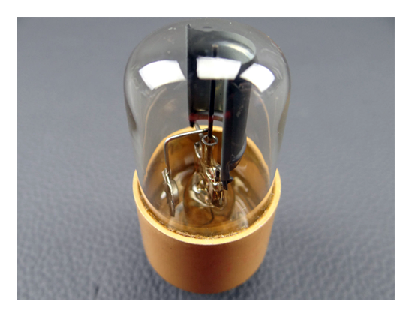
\includegraphics{RCA_IP39.eps}}\\
\caption{光電管 RCA IP39. }\label{fig:IP39} 
\end{center}
\end{minipage}
\end{figure}

光電管は,光をあてることのできる金属板と集電極が真空中に置かれ,それぞれ C 電極,A 電極と接続された構造をしている(図 \ref{fig:phototube}).
金属板に光をあてると,金属の表面から光電子が放出される.
これらが集電極に到達すれば,電極 A から電極 C にながれる電流として検出でき,電極に到達した光電子の量が電流の強さとなる.

ここで,金属版の電極 C に負電圧を印加すれば,放出された電子は陽極である集電極 A にあつまる.
逆に金属版を陽極として電圧を印加した場合,
放出された電子の持つ電極方向の運動エネルギーが,
電位差に逆らって電極に到達することによって失うエネルギー以上であるとき,はじめて集電極に到達し,電流が検知されることになる.
すなわち,集電極方向の電子の運動エネルギー $K = \frac{1}{2}m_{\rm e} v^2$ が $K \geq e |V|$ であるとき,電流が流れる.ただし $m_{\rm e}$ は電子の質量,$e$ は電子のもつ電荷の大きさ(電気素量)である.
金属板にあてる光を単色光とし,金属板を陽極として印加する電圧を高くしていくと,ある電圧で電流が 0 となる.
この電圧を,制止電圧という.
これは,単色光によって金属板から放出される電子の運動エネルギーの最大値 $K_{\max}$ と制止電圧 $V_0$ について $K_{\max} = e |V_0|$ が成り立つ状態にあるということである.

プランクは,黒体輻射の現象 --- 
熱せられた物体が放射する光の強さと振動数の関係 --- を説明するため,
光として放出されるエネルギーがとびとびの値をとる,エネルギー量子仮説を提唱した.
これによれば,振動数 $\nu$ の光により放出されるエネルギーの値は,$h \nu$ の整数倍 $n h \nu$ になる.
ただし $n$ は正の整数で,振動数 $\nu$ である光の強度を表す.
光電効果は輻射と逆の現象,つまり光が金属板にあたり,そのエネルギーが吸収されて電子が放出される現象である.
その電子の放出は,金属の面に光があたってから $10^{-9}$ 秒(1ナノ秒)より短い時間内におこり,照射から射出までに時間のおくれはない\cite{Arya-book-1974}.
つまりエネルギーの蓄積は行われていないと考えられるので,
金属板から放出される電子の運動エネルギーの最大値 $K_{\max}$ は,光のエネルギー量子の大きさに等しいと考えられる.
振動数 $\nu$ の光を照射したときの制止電圧が $V_0$ ならば,
\begin{eqnarray}\label{eq:1}
K_{\max} = e V_0 = h \nu + c
\end{eqnarray}
が成り立つことになる.
ここで,$c$ は電子が金属の束縛を逃れるために必要なエネルギーや,制止電圧の測定上のずれなどをふくむ定数(正または負)とする.

つまり,同じ光電管(の金属板)について,同じ回路で,照射する光の振動数 $\nu$ を変化させて制止電圧を測定すれば,振動数と制止電圧の関係から比例定数であるプランク定数 $h$ を求めることができる.

\section{実験}

まず,全体を通して使用する光電効果実験装置について,注意事項,および基本的な手順を付録 Appendix \ref{apdx:aparatus} で確認する.
そのうえで,実験 \ref{a} を行って実際に手順を確認する.
これら基本的な手順と測定方法を確認した後,実験 \ref{b} および \ref{c} を行う.


\subsection{光電流現象の確認,電極間印加電圧と光電流}\label{a}

波長を 1 つえらび,光電効果によって電流が流れることを確認せよ.
LED の点灯の ON/OFF は,LED の強度つまみを変化させる,
もしくは LED モジュールへの電力供給プラグを抜き差しすることで行う.
また,電圧調整つまみで制止電圧を変化させ,光電流が正または負で流れる値にする.

現象を確認し,また光電流がマイナスからプラスにかわる印加電圧を大まかに把握しておく.

\subsection{光の強度と光電流}\label{b}

LED の発光量が LED の強度つまみの位置によって,どのように変化するか,確認せよ.
次に,波長を 2 つえらび,LED の照射強度つまみの位置に対して光電流がどのように変化するか,
その関係を測定せよ.
照射強度を変化させる量は,目盛で確認できる 5 から 10\% 程度のきざみでよい.

\subsection{光の波長と阻止電圧}\label{c}

波長の異なる LED を光源として,各波長における阻止電圧を測定せよ.
そして振動数と阻止電圧がどのような関係になっているか,式 \ref{eq:1} の比例定数 $h$ と切片の定数 $c$ をもとめよ.
そして光電効果の原理にもとづき,それぞれを説明せよ.

定数 $h$ と $c$ の決定は,簡易的には,グラフを書いて直線を引き,そのグラフから傾きと切片を読み取ることで行うことができる.
実験がうまくいったかどうかは,この簡易な方法で確かめることができる.

\subsection{発展:最小二乗法}
正確に直線の傾きと切片を求めるには,最小二乗法 least squares method をもちいることができる.
どのような方法か,またなぜ一般に最小二乗法をもちいなければならないかを調べ,説明せよ.
また,MS Excel や関数電卓等で最小二乗法を使用する方法を調べ,測定の結果に適用し,定数の値を決定せよ.


\bibliographystyle{plain}
\bibliography{references}


\newpage
\appendix
\noindent
{\LARGE\bf 付録 Appendix}

\section{光電効果実験装置}\label{apdx:aparatus}

詳細はプランク定数測定装置 Planck's constant apparatus の付属説明書を参照せよ.
ここでは要点のみ説明する.

\begin{caution}
光電管に,測定以外で光があたらないよう注意すること.
強い光は C電極を劣化させ,感度が低下する,あるいは使用不可能となるおそれがある.
LED モジュールを装着している間以外は,かならずダミーのカバーを装着し,
LED モジュール,ダミーカバーは確実に装着されていることを確認すること.
\end{caution}

\subsection{各部の名称とはたらき}

光電管は,カバーにおおわれており,このカバー側面にある窓から LED の光を照射する(図 \ref{fig:phototube_cover}).
LED モジュールの波長記載ラベルが使用者正面を向くのが LED モジュールの正しい取り付け向きである.
LED は,モジュールの中に組み込まれている.
LED モジュールを取り付けるまえに,実験装置のソケットに LED モジュールのプラグを差し込み,照射強度調整つまみを回すと,点灯およびその明るさの変化を確認できる.

\begin{figure}[t]
\begin{center}
\scalebox{0.8}{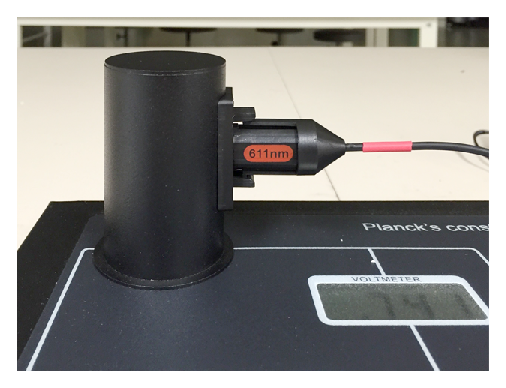
\includegraphics{LED_module_attach.eps}}\\
\caption{光電管カバーと LED モジュールカバー. }\label{fig:phototube_cover} 
\end{center}
\end{figure}

装置の上面パネルには,内蔵する電子回路の模式的な回路図が描かれている(図\ref{fig:controlpanel}).
実際にはデジタル式の電圧計,ナノアンペア電流計の回路を内蔵しているが,
この装置を使った実験では,表示される電圧および電流の値の誤差等はないものと考えて,
表示される値をそのまま測定値として使用することにする.
回路図の可変抵抗器(ポテンショメータ)は,実際にはコントロールパネル上の 2 つの印加電圧調整つまみで操作できる 2 つの可変抵抗器を直列に接続したもので構成されている.
この可変抵抗器は,電源装置(回路図では電池)から得られる一定の電圧を,抵抗の分圧によって調整し取り出すためにもちいられている.

\begin{figure}[t]
\begin{minipage}[t]{.5\textwidth}
\begin{center}
\scalebox{0.66}{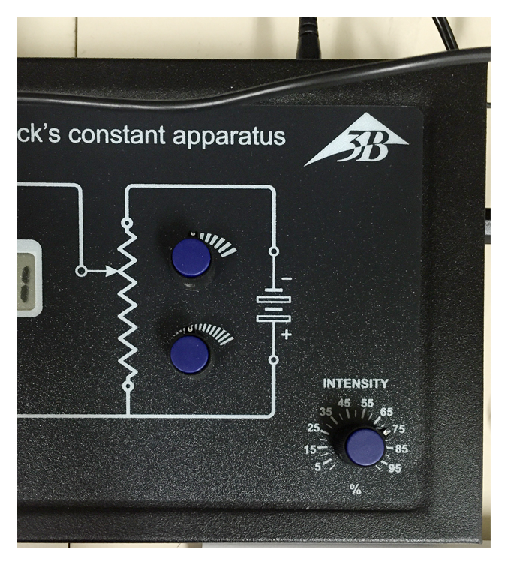
\includegraphics{control_panel.eps}}\\
\caption{装置上面パネルの印加電圧粗調整つまみ coarse nob(左上),微調整つまみ fine nob(左下).右下は LED 輝度の強度調整つまみ.}\label{fig:controlpanel} 
\end{center}
\end{minipage}
\hfill
\begin{minipage}[t]{.45\textwidth}
\begin{center}
\scalebox{0.75}{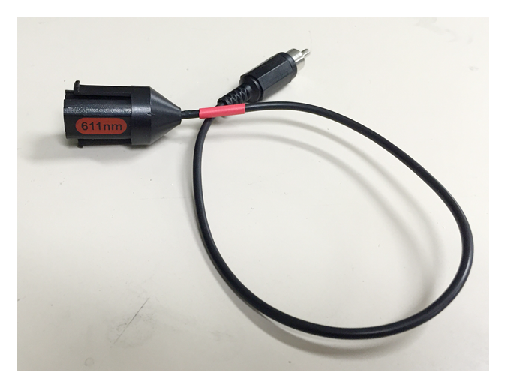
\includegraphics{LED_module.eps}}\\
\caption{LED モジュール. }\label{fig:LED_module} 
\end{center}
\end{minipage}
\end{figure}

この実験装置本体の電源回路に電力を供給するため,AC アダプタを接続する.

\subsection{基本的な操作}

制止電圧を測定するための手順は,以下のとおりである.
そのほかの測定も,これに準じて行う.
\begin{enumerate}
\item
装置本体に電源アダプタを接続し,
電源アダプタをコンセントに差し込んで電源を投入する.
装置のデジタル表示が点灯して動作していることを確認する.
\item
動作を安定させるため,実験を開始する前には 10 分程度あらかじめ電源を投入したままにして,
ウォーミングアップさせておく.
\item
強度つまみが 75\% 前後の位置で LED モジュールのプラグをソケットに接続し, LED が点灯することを確認する.
\item
ダミーカバーをとりはずし,LED モジュールを取り付ける.
モジュールの波長が記載されたラベルが前になるのが正しい向きである.
モジュールカバーが確実に取り付けられていることを確認する.
\item
電圧調整のつまみ両方を中央の位置にする.
\item
LED の発光を安定させるため,3 分程度待つ.
\item
印加電圧調整つまみで電流が $0$ となるよう調整する.
装置のナノアンペア電流計は,電流が $0$ のときマイナス `$-$' 符号なしの $0$ を表示する.

調整は,まず粗つまみで調整し,次に微つまみで微調整する.
\item
印加電圧を読み取る.
\item
測定がおわったら,LED モジュールを取りはずし,ダミーカバーをとりつける.
確実に取り付けられていることを確認する.
\item
波長をかえて測定をつづける場合は,LED モジュールをかえて,点灯の確認から以降を繰り返す.
\end{enumerate}

\end{document}
